\section{Datenbankschema}
\label{kap:dbschema}
In diesem Kapitel werden die Anforderungen an das Datenbankschema beschrieben. Anschliessend wird ein vereinfachtes Domänenmodell vorgestellt, das als Grundlage für die weiteren Kapitel dient. Danach folgen die Beschreibung der Lösungsansätze und deren Umsetzung. Diese bildet die Grundlage für die Erläuterungen des Kapitel~\ref{kap:vfs} -~\ref{kap:lsp}.

\subsection{Anforderungen}
\label{abb:anforderungen}
Das Ziel dieser Bachelorarbeit ist die Entwicklung einer generischen, datenmodellgetriebenen Anwendung zur Verwaltung von IoT-Konfigurationen. Die Anwendungslogik soll dabei vollständig aus einem definierten Datenmodell abgeleitet werden, sodass Anpassungen im Quellcode vermieden werden. Daraus ergeben sich drei Anforderungen an das Datenbankschema: Erstens müssen Einstiegspunkte im Schema definiert werden, damit die Anwendung erkennt, wo der Verwaltungsprozess beginnt. Zweitens muss das Schema zusätzliche Validierungen unterstützen, da die verwendete Datenbanktechnologie Selva nur grundlegende Datentyp-Prüfungen bereitstellt. Drittens soll es möglich sein, zusätzliche Informationen wie beispielsweise Blattknoten oder potenzielle zyklische Verweise aus dem Schema abzuleiten, ohne dass diese im Schema definiert werden müssen.

\subsection{Domänenmodell}
\label{abb:domaenenmodell}
Das in Abschnitt~\ref{abb:tech} beschriebene Domänenmodell ist zu komplex, um es unverändert in der entwickelten Lösung zu verwenden. Deshalb wird zunächst ein vereinfachtes Modell definiert, das für die Umsetzung geeignet ist. Die Übertragbarkeit auf das Domänenmodell der Monidas-Plattform wird in Kapitel~\ref{kap:eva} untersucht.

Das für diese Arbeit verwendete Domänenmodell ist in Abbildung~\ref{ab:con} dargestellt und bildet ein typisches Szenario aus dem E-Commerce-Bereich ab. Das Modell besteht aus den fünf Entitäten: \textit{Customer}, \textit{Address}, \textit{Order}, \textit{LineItem} und \textit{Product}. Ein \textit{Customer} (Kunde) verfügt über Angaben wie Vorname, Nachname und eine E-Mail-Adresse. Jeder Kunde besitzt mehrere Adressen (\textit{Address}) und kann mehrere Bestellungen (\textit{Order}) tätigen. Eine Adresse umfasst die Strasse, Stadt sowie das Land und gehört eindeutig zu einem Kunden. Jede Bestellung besitzt eine Rechnungsadresse (\textit{billingAddress}) und optional eine Lieferadresse (\textit{shippingAddress}). Eine Bestellung besteht aus mindestens einer Bestellposition (\textit{LineItem}), welche jeweils ein Produkt (\textit{Product}) mit einer definierten Menge und einem Einzelpreis referenziert. Ein Produkt enthält eine eindeutige Beschreibung sowie einen Preis.

\begin{figure}[H]
    \centering
    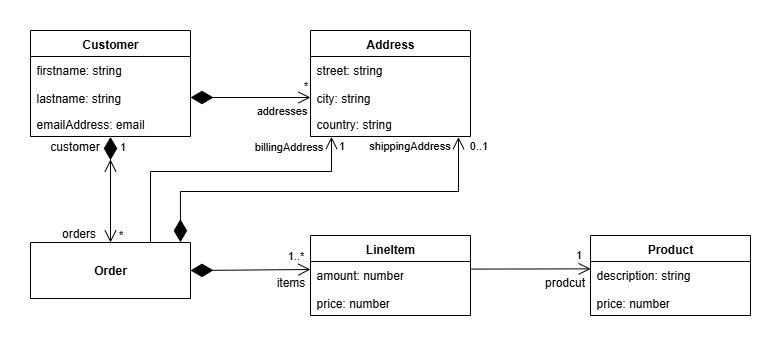
\includegraphics[width=0.8\linewidth]{Bsp_UML.png}
    \caption{Vereinfachtes Domänenmodell im E-Commerce-Kontext}
    \label{fig:uml_domaenenmodell}
\end{figure}

\subsection{Schemaerweiterungen}
Um die Anforderungen der Anwendung erfüllen zu können, mussten Erweiterungen am bestehenden Schema vorgenommen werden. Diese umfassen die Definition von Einstiegspunkten (Roots), Bedingungen (Constraints) sowie die dynamische Ableitung zusätzlicher Informationen.

\label{ab:con}
\subsubsection{Roots}
Unter dem Begriff «Roots» werden die im Schema definierten Einstiegspunkte verstanden. Diese bestimmen, bei welchen Entitäten die Navigation im virtuellen Filesystem beginnt. Für jeden Root wird ein Label festgelegt, das im Filesystem als Ordnername angezeigt wird. Dieses Label wird direkt im Schema definiert und kann unabhängig vom Namen der Entität frei gewählt werden.

Im E-Commerce-Domänenmodell (siehe Abbildung \ref{fig:uml_domaenenmodell}) könnten beispielsweise die Entitäten \textit{Customer} mit dem Label \textit{Customers} und \textit{Product} mit dem Label \textit{Products} als Roots definiert werden.

\subsubsection{Constraints}
Unter «Constraints» werden in dieser Thesis Bedingungen verstanden, die das Standardverhalten der Applikation gezielt ergänzen oder einschränken. Sie stellen sicher, dass die Daten bestimmte Anforderungen erfüllen und inhaltlich konsistent bleiben. Diese Bedingungen werden ausschliesslich von der Anwendungslogik geprüft und nicht von der Datenbank selbst.

Das Standardverhalten der Applikation sieht vor, dass neue Objekte direkt innerhalb ihres übergeordneten Knotens erstellt werden. Dieses Verhalten folgt einer Parent-Child-Hierarchie. Das Referenzieren eines bereits bestehenden Objekts ist standardmässig deaktiviert. Mit „Referenzieren“ wird in dieser Arbeit verstanden, dass beispielsweise bei einer Bestellung keine neue Adresse erstellt, sondern eine bereits existierende Adresse zugeordnet wird.

Werden jedoch zusätzliche Bedingungen benötigt, um das Standardverhalten gezielt zu erweitern, stehen die folgenden Constraints zur Verfügung: Pflichtfeld (notNull), bidirektionale Verknüpfung (bidirektional), Verbot der Erstellung neuer Objekte (denyCreation) und Erlaubnis zum Referenzieren bestehender Objekte (allowReference). Zur Veranschaulichung dieser Constraints dient folgendes Beispiel aus dem E-Commerce-Domänenmodell:

Beim Erstellen eines neuen Kunden ist die Angabe einer E-Mail-Adresse zwingend erforderlich (notNull), andernfalls ist das Speichern nicht möglich. Anschliessend erstellt der Kunde zwei Adressen, beispielsweise eine Heimadresse und eine Arbeitsadresse, welche eindeutig diesem Kunden zugeordnet sind. Möchte der Kunde eine Bestellung tätigen, ist dafür zwingend die Angabe einer Rechnungsadresse (billingAddress) erforderlich (notNull). Innerhalb der Bestellung ist das Erstellen einer neuen Rechnungsadresse technisch nicht möglich, da dies explizit deaktiviert wurde (denyCreation). Stattdessen muss eine bereits vorhandene Adresse ausgewählt werden (allowReference), beispielsweise die zuvor erstellte Arbeitsadresse. Darüber hinaus muss jede Bestellung mindestens eine Bestellposition enthalten (notNull). Diese Bestellposition wird direkt im Kontext der Bestellung erstellt und muss zwingend auf ein bereits bestehendes Produkt (Product) verweisen (allowReference, denyCreation). Optional kann zudem eine Lieferadresse angegeben werden. Diese Lieferadresse wird direkt im Kontext der Bestellung erstellt und existiert ausschliesslich dort. Das Referenzieren bereits bestehender Adressen, beispielsweise der Heim- oder Arbeitsadresse, ist hierbei technisch deaktiviert und daher nicht möglich (Standardverhalten).

\subsubsection{Schema Analyse}
\label{sec:dynamischerAb}
Die zuvor beschriebenen Schemaerweiterungen wie Constraints und Roots werden statisch definiert. Eine weitere Information, nämlich ob ein Referenzfeld zu einem Blattknoten (\textit{isLeaf}) führt, lässt sich hingegen durch eine Schema-Analyse ableiten. Ein Blattknoten bezeichnet hierbei einen Knoten, dessen Entitätstyp keine weiteren ausgehenden Referenzen besitzt. Diese ermittelte Information wird genutzt, um Darstellungs- und Bearbeitungslogiken innerhalb des virtuellen Filesystems zu steuern. Die konkrete Verwendung wird detailliert in Kapitel~\ref{kap:vfs} erläutert. Dies wird direkt im Schema ergänzt, wodurch sich der Modellierungsaufwand reduziert und die Flexibilität für Erweiterungen steigt.

Für die Schema-Analyse wird das Schema als gerichteter Graph interpretiert. Entitätstypen wie \textit{Customer}, \textit{Order}, \textit{Address}, \textit{LineItem} und \textit{Product} bilden dabei die Knoten, während Referenzfelder wie \textit{addresses}, \textit{billingAddress}, \textit{shippingAddress}, \textit{customer}, \textit{items} und \textit{product} die gerichteten Kanten darstellen. Zur Traversierung des Graphen wird der Algorithmus der Tiefensuche (Depth-First Search, DFS) verwendet. Dabei handelt es sich um einen Graphen-Algorithmus, der von einem Startknoten ausgehend zunächst einen Pfad vollständig verfolgt, bevor zurückgegangen und der nächste Pfad untersucht wird. 

\begin{figure}[H]
    \centering
    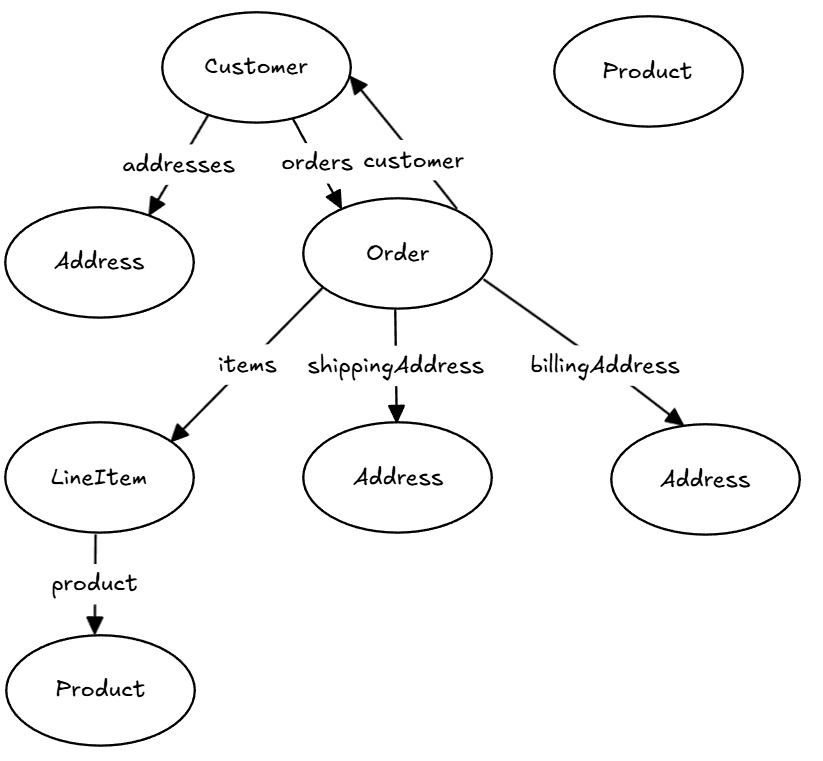
\includegraphics[width=0.8\linewidth]{dag.png}
    \caption{Gerichtete Graphdarstellung des E-Commerce-Datenbankschemas}
    \label{fig:dag}
\end{figure}
\newpage

Im Rahmen der Lösungsfindung wurden weitere Ansätze zur Informationsableitung geprüft. Einer dieser Ansätze bestand darin, sämtliche möglichen URIs bereits im Vorfeld aus dem Schema abzuleiten. Ein URI (Uniform Resource Identifier) bezeichnet hierbei einen eindeutigen Pfad, der sich aus der Abfolge von Referenzfeldern (gerichteten Kanten) und Instanzen von Entitätstypen (Knoten) zusammensetzt. Eine Instanz bezeichnet dabei ein konkretes Datenobjekt, das auf Basis einer im Schema definierten Entität erzeugt wurde. Beispielsweise ergibt sich ein URI aus einer Abfolge wie:

\begin{center}
\texttt{Customers/\{customerId\}/Orders/\{orderId\}}
\end{center}

Ziel dieses Ansatzes war es, alle gültigen URI-Muster im Vorfeld zu ermitteln, um URIs zur Laufzeit validieren zu können. Dieses Vorgehen ist allerdings nur geeignet, wenn im Schema keine Zyklen auftreten. Sobald zyklische Referenzen vorhanden sind, entstehen theoretisch unendlich viele URI-Kombinationen. Daher lässt sich dieser Ansatz bei zyklischen Schemata nicht allgemein anwenden.

Ein weiterer untersuchter Ansatz bestand darin, die genaue Pfadtiefe eines URI bereits im Voraus zu ermitteln. Da jedoch eine vollständige Abbildung aller möglichen URIs vorab nicht realisierbar war und sich die Pfadtiefe ohnehin einfach direkt aus dem URI während einer Anfrage ableiten lässt, erwies sich dieser Ansatz letztlich als nicht zielführend und wurde verworfen.
%hasPossbileCycle
%\subsection{Bereitstellung und Zugriff}

\subsection{Umsetzung}

\subsubsection{Roots und Constraints}
Die Definition von Einstiegspunkten („Roots“) sowie zusätzlichen Validierungen („Constraints“) erfordert eine Erweiterung der ursprünglichen TypeScript-Typdefinition aus der Colombalink-Bibliothek. Für die Umsetzung wurde das bestehende Schema aus der Colombalink-Bibliothek angepasst. Dabei wurde die Typdefintion Schema erweitert, um die Definition von Roots und Constraints zu ermöglichen. Die dafür notwendigen TypeScript-Features wie Omit, Intersection Types, Union Types und Generics stellten sicher, dass diese Erweiterung umgesetzt werden konnte~\cite{typescript:handbook}. Das Ergebnis ist ein erweitertes Schema, das den Anforderungen aus Abschnitt~\ref{abb:anforderungen} entspricht. Die genaue technische Umsetzung befindet sich im Anhang in Listing~\ref{lst:extended-schema}.

Im vorherigen Abschnitt wurde bereits erläutert, wie im konkreten E-Commerce-Domänen\-modell die Entitäten \textit{Customer} und \textit{Product} als Roots definiert wurden, sowie welche Constraints für die Entität \textit{Order} gesetzt wurden. Im nachfolgenden Listing~\ref{lst:con} ist dargestellt, wie dies im erweiterten Schema definiert werden können.

\newpage
\lstinputlisting[
caption={Definition von Roots und Constraints im erweiterten Schema},
label={lst:con},
style=customtypescript
]{listings/con.json}

\newpage
\subsubsection{Schema Analyse}
Die technische Umsetzung der Schema-Analyse erfolgt mithilfe einer rekursiven Tiefensuche. Ausgangspunkte der Traversierung sind die zuvor definierten Einstiegspunkte (\textit{Customer} und \textit{Product}, siehe Abschnitt~\ref{ab:con}).

Während der Tiefensuche wird jeder besuchte Entitätstyp (Knoten) erfasst. Wird ein bereits besuchter Knoten erneut erreicht, deutet dies auf einen möglichen Zyklus hin und die weitere Traversierung entlang dieses Pfades wird beendet. Hat ein referenzierter Knoten keine weiteren ausgehenden Referenzen, wird das Feld \texttt{isLeaf} gesetzt, um ihn als Blattknoten zu kennzeichnen.

Das Ergebnis der Schema-Analyse für das E-Commerce-Schema ist in Tabelle~\ref{tab:schema-analyse-dfs} dargestellt. Der zugehörige Code befindet sich im Anhang (Listing~\ref{lst:extendSchemaDFS}).

\begin{table}[H]
  \centering
  \begin{tabular}{lllc}
    \toprule
    \textbf{Ausgangsknoten} & \textbf{Referenz (Kante)} & \textbf{Zielknoten} & \textbf{isLeaf}\\ 
    \midrule
    Product & – & – & – \\[4pt]
    Customer & addresses & Address & Ja \\[4pt]
    Customer & orders & Order & Nein \\[4pt]
    Order & billingAddress & Address & Ja \\[4pt]
    Order & shippingAddress & Address & Ja \\[4pt]
    Order & items & LineItem & Nein \\[4pt]
    LineItem & product & Product & Ja \\[4pt]
    Order & customer & Customer & Nein \\ 
    \bottomrule
  \end{tabular}
  \caption{Ergebnis der Schema-Analyse mit DFS für das E-Commerce-Schema}
  \label{tab:schema-analyse-dfs}
\end{table}


